\documentclass[12pt, a4paper]{book}

\usepackage[T1]{fontenc}
\usepackage[utf8]{inputenc}
\usepackage[charter, cal=cmcal]{mathdesign}
\usepackage[scaled=0.92]{helvet}
\usepackage{geometry}
\geometry{a4paper, top=30mm, bottom=30mm, inner=32mm, outer=25mm, marginparwidth=18mm}

\usepackage{amsmath, amsthm}
\usepackage[version=4]{mhchem}
\usepackage{graphicx}
\usepackage[dvipsnames,svgnames,table]{xcolor}
\usepackage{tikz}
\usetikzlibrary{arrows.meta, shapes.geometric, positioning, calc, backgrounds}
\usepackage{pgfplots}
\pgfplotsset{compat=1.18}
\usepackage{tcolorbox}
\tcbuselibrary{skins, breakable, theorems}
\usepackage{titlesec}
\usepackage{fancyhdr}
\usepackage{enumitem}
\usepackage{booktabs}
\usepackage{array}
\usepackage{parskip}
\usepackage{siunitx}
\usepackage[colorlinks=true, linkcolor=BrickRed,
            urlcolor=NavyBlue, citecolor=ForestGreen]{hyperref}

% ── Colours (Journey 4 — deep teal / slate) ───────────────────────────────────
\definecolor{JourneyColor}{HTML}{1A5276}
\definecolor{ModuleColor}{HTML}{2E86C1}
\definecolor{PuzzleColor}{HTML}{145A32}
\definecolor{DiscoveryColor}{HTML}{B7950B}
\definecolor{WarningColor}{HTML}{C0392B}
\definecolor{ProblemColor}{HTML}{4A235A}
\definecolor{ReflectColor}{HTML}{117A65}
\definecolor{HistoryColor}{HTML}{6E2F1A}
\definecolor{IonicColor}{HTML}{922B21}
\definecolor{CovalentColor}{HTML}{1A5276}
\definecolor{MetallicColor}{HTML}{784212}
\definecolor{VdWColor}{HTML}{1E8449}

% ── Boxes ─────────────────────────────────────────────────────────────────────
\newtcolorbox{puzzlebox}[1][]{enhanced,breakable,
  colback=PuzzleColor!6,colframe=PuzzleColor,fonttitle=\bfseries\sffamily,
  title={The Puzzle},attach boxed title to top left={yshift=-2mm,xshift=6mm},
  boxed title style={colback=PuzzleColor},borderline west={3pt}{0pt}{PuzzleColor},#1}

\newtcolorbox{discoverybox}[1][]{enhanced,breakable,
  colback=DiscoveryColor!8,colframe=DiscoveryColor,fonttitle=\bfseries\sffamily,
  title={Discovery},attach boxed title to top left={yshift=-2mm,xshift=6mm},
  boxed title style={colback=DiscoveryColor},borderline west={3pt}{0pt}{DiscoveryColor},#1}

\newtcolorbox{problembox}[1][]{enhanced,breakable,
  colback=ProblemColor!5,colframe=ProblemColor,fonttitle=\bfseries\sffamily,
  title={Problems},attach boxed title to top left={yshift=-2mm,xshift=6mm},
  boxed title style={colback=ProblemColor},borderline west={3pt}{0pt}{ProblemColor},#1}

\newtcolorbox{deepbox}[1][]{enhanced,breakable,
  colback=JourneyColor!5,colframe=JourneyColor,fonttitle=\bfseries\sffamily,
  title={Deep Problems},attach boxed title to top left={yshift=-2mm,xshift=6mm},
  boxed title style={colback=JourneyColor},borderline west={4pt}{0pt}{JourneyColor},#1}

\newtcolorbox{historybox}[1][]{enhanced,breakable,
  colback=HistoryColor!7,colframe=HistoryColor!60,fonttitle=\bfseries\sffamily\small,
  title={Historical Note},attach boxed title to top left={yshift=-2mm,xshift=6mm},
  boxed title style={colback=HistoryColor!80},#1}

\newtcolorbox{reflectionbox}[1][]{enhanced,breakable,
  colback=ReflectColor!6,colframe=ReflectColor,fonttitle=\bfseries\sffamily,
  title={Reflection},attach boxed title to top left={yshift=-2mm,xshift=6mm},
  boxed title style={colback=ReflectColor},borderline west={3pt}{0pt}{ReflectColor},#1}

\newtcolorbox{namedconcept}[2][]{enhanced,
  colback=ModuleColor!6,colframe=ModuleColor,fonttitle=\bfseries\sffamily\large,
  title={#2},attach boxed title to top left={yshift=-2mm,xshift=6mm},
  boxed title style={colback=ModuleColor},#1}

% ── Section formatting ────────────────────────────────────────────────────────
\titleformat{\chapter}[display]
  {\normalfont\sffamily\huge\bfseries\color{JourneyColor}}
  {\textcolor{JourneyColor!60}{\chaptertitlename\ \thechapter}}{10pt}{\Huge}
  [\vspace{2pt}\textcolor{JourneyColor}{\titlerule[1.5pt]}]
\titleformat{\section}
  {\normalfont\sffamily\Large\bfseries\color{ModuleColor}}
  {\thesection}{1em}{}[\textcolor{ModuleColor!40}{\titlerule[0.6pt]}]
\titleformat{\subsection}
  {\normalfont\sffamily\large\bfseries\color{JourneyColor!80}}{\thesubsection}{1em}{}
\titleformat{\subsubsection}
  {\normalfont\sffamily\normalsize\bfseries}{\thesubsubsection}{1em}{}

\pagestyle{fancy}
\fancyhf{}
\fancyhead[LE]{\small\sffamily\textcolor{JourneyColor}{\leftmark}}
\fancyhead[RO]{\small\sffamily\textcolor{ModuleColor}{\rightmark}}
\fancyfoot[C]{\small\thepage}
\renewcommand{\headrulewidth}{0.4pt}

\newcommand{\newterm}[1]{\textit{\textcolor{DiscoveryColor}{#1}}}
\newcommand{\important}[1]{\textcolor{ModuleColor}{\textbf{#1}}}

% Journey 4 opener
\newcommand{\journeyopener}{%
\begin{tcolorbox}[enhanced,
  colback=JourneyColor!10, colframe=JourneyColor,
  width=\textwidth, arc=5pt]
\centering\sffamily
{\large\bfseries\color{JourneyColor} Journey Four}\\[4pt]
{\normalsize\color{ModuleColor}\textbf{The Bond: Why Atoms Stick Together}}\\[6pt]
{\small\color{JourneyColor!70}
Six modules $\cdot$ $\sim$65 pages $\cdot$
From the puzzle of attraction to the continuum of bonding}
\end{tcolorbox}}

% ══════════════════════════════════════════════════════════════════════════════
\begin{document}
\setcounter{chapter}{3}
\chapter[Journey 4 --- The Bond: Why Atoms Stick Together]
        {Journey Four\\[8pt]
         \textcolor{ModuleColor}{\large The Bond: Why Atoms Stick Together}}

\journeyopener
\vspace{1em}

% ── Journey 4 module map ──────────────────────────────────────────────────────
\begin{center}
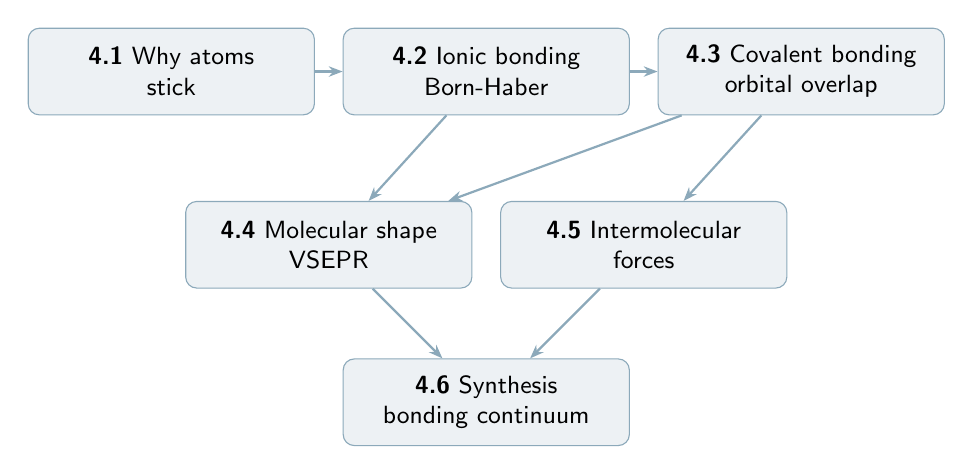
\begin{tikzpicture}[
  every node/.style={font=\sffamily\small, align=center},
  modbox/.style={draw=JourneyColor!50, fill=JourneyColor!8,
    rounded corners=4pt, minimum width=3.6cm, minimum height=1.1cm,
    text width=3.4cm},
  arr/.style={-{Stealth[length=5pt]}, thick, JourneyColor!50}
]
  \node[modbox] (m1) at (0,0)   {\textbf{4.1} Why atoms\\stick};
  \node[modbox] (m2) at (4.0,0) {\textbf{4.2} Ionic bonding\\Born-Haber};
  \node[modbox] (m3) at (8.0,0) {\textbf{4.3} Covalent bonding\\orbital overlap};
  \node[modbox] (m4) at (2.0,-2.2) {\textbf{4.4} Molecular shape\\VSEPR};
  \node[modbox] (m5) at (6.0,-2.2) {\textbf{4.5} Intermolecular\\forces};
  \node[modbox] (m6) at (4.0,-4.2) {\textbf{4.6} Synthesis\\bonding continuum};
  \draw[arr] (m1)--(m2); \draw[arr] (m2)--(m3);
  \draw[arr] (m2)--(m4); \draw[arr] (m3)--(m4);
  \draw[arr] (m3)--(m5); \draw[arr] (m4)--(m6); \draw[arr] (m5)--(m6);
\end{tikzpicture}
\end{center}

\vspace{1em}
\setcounter{section}{0}

% ══════════════════════════════════════════════════════════════════════════════
\section{Module 4.1 --- The Puzzle of Bonding: Why Do Atoms Stick?}
\label{sec:mod4.1}

\subsection*{Motivation}

Atoms are electrically neutral.
Molecules are collections of neutral atoms held together.
This is puzzling.

Why would two neutral hydrogen atoms attract each other
at all?
Neutral objects, by classical electrostatics, exert no
net force on each other.
Yet \ce{H2} is more stable than two separate H atoms
by 432 kJ/mol --- a large, measurable energy.

Something is wrong with the classical picture.
The something is quantum mechanics.

This module poses the bonding puzzle precisely,
surveys the landscape of bond types,
and asks the question that the next five modules will answer:
\emph{what physical mechanism stabilises a molecule
relative to its constituent atoms?}

\subsection{The Energy Landscape of a Bond}

When two atoms approach each other, their potential
energy changes.
The key observations are:

\begin{enumerate}[nosep, leftmargin=2em]
  \item At large separation: essentially zero interaction.
  \item At intermediate distance: the energy \emph{decreases} ---
        the atoms attract. This is the bonded region.
  \item At very short distance: the energy \emph{increases sharply} ---
        nuclear-nuclear and electron-electron repulsion dominates.
  \item There is a \newterm{bond length} $r_0$ where the
        energy is minimum --- the equilibrium geometry.
  \item The depth of the minimum is the \newterm{bond dissociation
        energy} $D_e$.
\end{enumerate}

\begin{center}
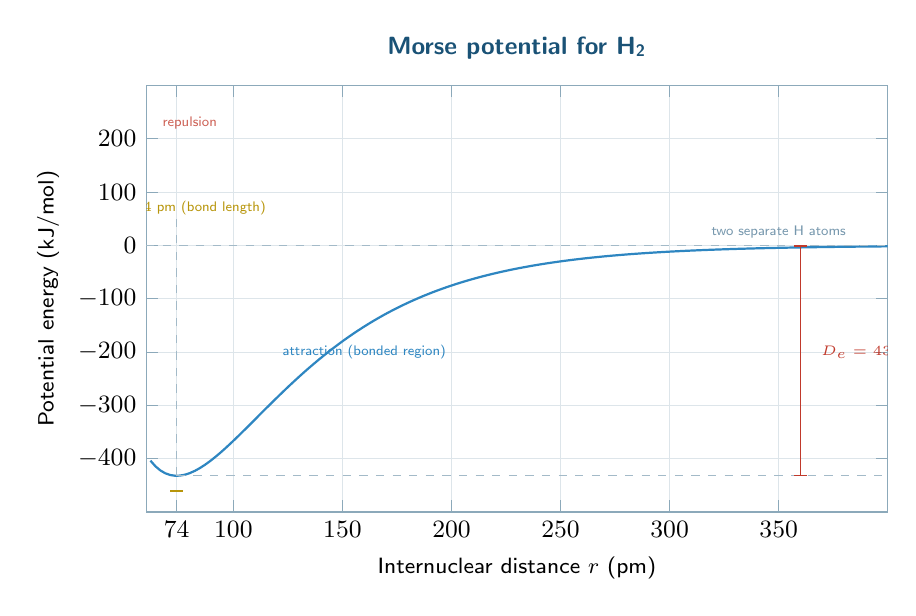
\begin{tikzpicture}[every node/.style={font=\sffamily\small}]
  \begin{axis}[
    width=11cm, height=7cm,
    xlabel={Internuclear distance $r$ (pm)},
    ylabel={Potential energy (kJ/mol)},
    xmin=60, xmax=400,
    ymin=-500, ymax=300,
    xtick={74,100,150,200,250,300,350},
    ytick={-400,-300,-200,-100,0,100,200},
    grid=both,
    grid style={line width=0.3pt, draw=JourneyColor!15},
    axis line style={color=JourneyColor!50},
    tick style={color=JourneyColor!50},
    title style={font=\sffamily\small\bfseries, color=JourneyColor},
    title={Morse potential for \ce{H2}},
    label style={font=\sffamily\footnotesize}
  ]
    % Morse potential: V(r) = De*(1-exp(-a*(r-re)))^2 - De
    % For H2: De ~ 432 kJ/mol, re ~ 74 pm, a = 0.019 pm^{-1}
    \addplot[thick, color=ModuleColor, domain=62:400, samples=150]
      {432*(1-exp(-0.019*(x-74)))^2 - 432};

    % Annotations
    \draw[dashed, thin, JourneyColor!40] (axis cs:74,-432) -- (axis cs:74,50);
    \draw[dashed, thin, JourneyColor!40] (axis cs:74,-432) -- (axis cs:400,-432);
    \draw[dashed, thin, JourneyColor!40] (axis cs:60,0) -- (axis cs:400,0);

    % r0 annotation
    \draw[{|}-{|}, thin, DiscoveryColor]
      (axis cs:74,-460) -- (axis cs:74,-460);
    \node[font=\sffamily\tiny, text=DiscoveryColor]
      at (axis cs:74,70) {$r_0 = 74$ pm (bond length)};

    % De annotation
    \draw[{|}-{|}, thin, WarningColor]
      (axis cs:360,-432) -- (axis cs:360,0);
    \node[font=\sffamily\tiny, text=WarningColor, anchor=west]
      at (axis cs:365,-200) {$D_e = 432$ kJ/mol (bond energy)};

    % Repulsion label
    \node[font=\sffamily\tiny, text=WarningColor!80]
      at (axis cs:80,230) {repulsion};

    % Attraction label
    \node[font=\sffamily\tiny, text=ModuleColor]
      at (axis cs:160,-200) {attraction (bonded region)};

    % Asymptote label
    \node[font=\sffamily\tiny, text=JourneyColor!60]
      at (axis cs:350,25) {two separate H atoms};
  \end{axis}
\end{tikzpicture}
\end{center}

\vspace{0.4em}

The Morse potential shown above is an empirical fit.
The actual quantum mechanical calculation
(solving the Schr\"{o}dinger equation for \ce{H2})
reproduces this curve from first principles.
The stabilisation comes entirely from electron delocalization
--- the quantum mechanical sharing of electrons between nuclei.

\begin{puzzlebox}
Consider two hydrogen atoms, each with one electron.

\begin{enumerate}[label=(\alph*), leftmargin=*]
  \item Classically, two neutral atoms exert no force on
        each other at large distance.
        Yet as they approach, there is an attractive force.
        List all the electrostatic interactions present
        when the two atoms are a distance $r$ apart.
        (There are four: two attractive and two repulsive.)

  \item As the atoms approach, the total Coulomb energy
        can be written as:
        \[
          V = \underbrace{-\frac{e^2}{4\pi\varepsilon_0 r_{1A}}
                          -\frac{e^2}{4\pi\varepsilon_0 r_{1B}}
                          -\frac{e^2}{4\pi\varepsilon_0 r_{2A}}
                          -\frac{e^2}{4\pi\varepsilon_0 r_{2B}}}_{\text{electron-nucleus}}
              +\underbrace{\frac{e^2}{4\pi\varepsilon_0 r_{12}}}_{\text{e-e}}
              +\underbrace{\frac{e^2}{4\pi\varepsilon_0 R}}_{\text{nuc-nuc}}
        \]
        where $R$ is the internuclear distance.
        At the equilibrium bond length, this potential
        energy is \emph{more negative} than for two
        separate atoms.
        But the electrons are being repelled from each other
        (positive $r_{12}$ term).
        What must be true about the electron-nucleus
        attraction terms to make the molecule stable?

  \item A classical electron sitting exactly midway between
        two protons would be attracted to both.
        A quantum mechanical electron can be \emph{simultaneously
        near both protons} --- it is smeared across the bond.
        Why would this quantum delocalization lower
        the electron's energy?
        (Hint: recall the particle-in-a-box.
        A longer box has lower ground-state energy.)

  \item Noble gas atoms (He, Ne, Ar) form essentially
        no chemical bonds.
        Other atoms do.
        Using the electron configuration language from
        Journey~2, what distinguishes noble gas atoms
        from bonding atoms?
\end{enumerate}
\end{puzzlebox}

\subsection{The Four Types of Chemical Bond}

Bonds arise from different mechanisms of electron sharing
or transfer.
The four main types form a continuum based on what
happens to the valence electrons.

\begin{center}
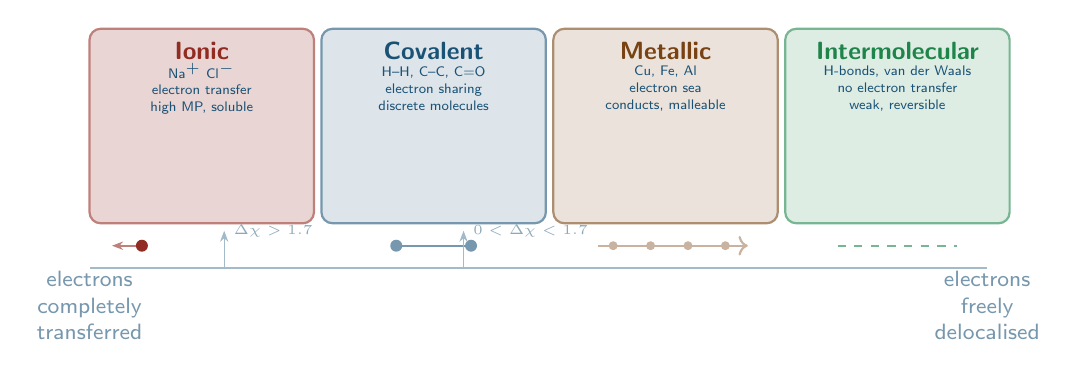
\begin{tikzpicture}[every node/.style={font=\sffamily\small, align=center},
                    scale=0.95]

  % Central axis: electron behaviour
  \draw[thick, JourneyColor!40] (0,0) -- (12,0);
  \node[font=\sffamily\footnotesize, text=JourneyColor!60]
    at (0,-0.5) {electrons\\completely\\transferred};
  \node[font=\sffamily\footnotesize, text=JourneyColor!60]
    at (12,-0.5) {electrons\\freely\\delocalised};

  % Four bond types
  \begin{scope}[xshift=0.5cm]
    \fill[IonicColor!20, rounded corners=4pt]
      (-0.5,0.6) rectangle (2.5,3.2);
    \draw[thick, IonicColor!60, rounded corners=4pt]
      (-0.5,0.6) rectangle (2.5,3.2);
    \node[font=\sffamily\small\bfseries, text=IonicColor]
      at (1.0,2.9) {Ionic};
    \node[font=\sffamily\tiny, text=JourneyColor]
      at (1.0,2.4) {Na$^+$ Cl$^-$\\electron transfer\\high MP, soluble};
    \draw[{Stealth[length=4pt]}-, thick, IonicColor!60]
      (-0.2,0.3) -- (0.2,0.3);
    \fill[IonicColor] (0.2,0.3) circle (0.08cm);
  \end{scope}

  \begin{scope}[xshift=3.6cm]
    \fill[CovalentColor!15, rounded corners=4pt]
      (-0.5,0.6) rectangle (2.5,3.2);
    \draw[thick, CovalentColor!60, rounded corners=4pt]
      (-0.5,0.6) rectangle (2.5,3.2);
    \node[font=\sffamily\small\bfseries, text=CovalentColor]
      at (1.0,2.9) {Covalent};
    \node[font=\sffamily\tiny, text=JourneyColor]
      at (1.0,2.4) {H--H, C--C, C=O\\electron sharing\\discrete molecules};
    \fill[CovalentColor!60] (0.5,0.3) circle (0.08cm);
    \fill[CovalentColor!60] (1.5,0.3) circle (0.08cm);
    \draw[thick, CovalentColor!60] (0.5,0.3) -- (1.5,0.3);
  \end{scope}

  \begin{scope}[xshift=6.7cm]
    \fill[MetallicColor!15, rounded corners=4pt]
      (-0.5,0.6) rectangle (2.5,3.2);
    \draw[thick, MetallicColor!60, rounded corners=4pt]
      (-0.5,0.6) rectangle (2.5,3.2);
    \node[font=\sffamily\small\bfseries, text=MetallicColor]
      at (1.0,2.9) {Metallic};
    \node[font=\sffamily\tiny, text=JourneyColor]
      at (1.0,2.4) {Cu, Fe, Al\\electron sea\\conducts, malleable};
    \foreach \x in {0.3,0.8,1.3,1.8} {
      \fill[MetallicColor!40] (\x,0.3) circle (0.06cm);
    }
    \draw[thick, MetallicColor!40, ->] (0.1,0.3) -- (2.1,0.3);
  \end{scope}

  \begin{scope}[xshift=9.8cm]
    \fill[VdWColor!15, rounded corners=4pt]
      (-0.5,0.6) rectangle (2.5,3.2);
    \draw[thick, VdWColor!60, rounded corners=4pt]
      (-0.5,0.6) rectangle (2.5,3.2);
    \node[font=\sffamily\small\bfseries, text=VdWColor]
      at (1.0,2.9) {Intermolecular};
    \node[font=\sffamily\tiny, text=JourneyColor]
      at (1.0,2.4) {H-bonds, van der Waals\\no electron transfer\\weak, reversible};
    \draw[dashed, thick, VdWColor!60] (0.2,0.3) -- (1.8,0.3);
  \end{scope}

  % Delta-chi axis
  \draw[-{Stealth[length=4pt]}, thin, JourneyColor!40]
    (1.8,0) -- (1.8,0.5)
    node[right, font=\sffamily\tiny, text=JourneyColor!50]
      {$\Delta\chi > 1.7$};
  \draw[-{Stealth[length=4pt]}, thin, JourneyColor!40]
    (5.0,0) -- (5.0,0.5)
    node[right, font=\sffamily\tiny, text=JourneyColor!50]
      {$0 < \Delta\chi < 1.7$};

\end{tikzpicture}
\end{center}

\vspace{0.4em}

The distinction between bond types is not absolute.
A bond between atoms of very different electronegativity
(e.g.\ Na--Cl, $\Delta\chi = 2.1$) is primarily ionic.
A bond between identical atoms (H--H, $\Delta\chi = 0$)
is purely covalent.
Between these extremes lies a continuum of polarity.

\begin{center}
\small
\begin{tabular}{lllcl}
\toprule
Bond type & Example & $\Delta\chi$ & Charge separation & Character \\
\midrule
Pure covalent   & \ce{H-H}  & 0.0 & none & nonpolar \\
Polar covalent  & \ce{H-Cl} & 0.9 & partial ($\delta+$/$\delta-$) & polar \\
Polar covalent  & \ce{H-O}  & 1.4 & large partial & very polar \\
Ionic           & \ce{Na-Cl} & 2.1 & nearly full & ionic \\
Very ionic      & \ce{Cs-F} & 3.3 & full transfer & ionic \\
\bottomrule
\end{tabular}
\end{center}

\subsection{What Makes a Bond Strong?}

Bond energies span an enormous range.
Understanding the factors is essential for predicting
reactivity.

\begin{center}
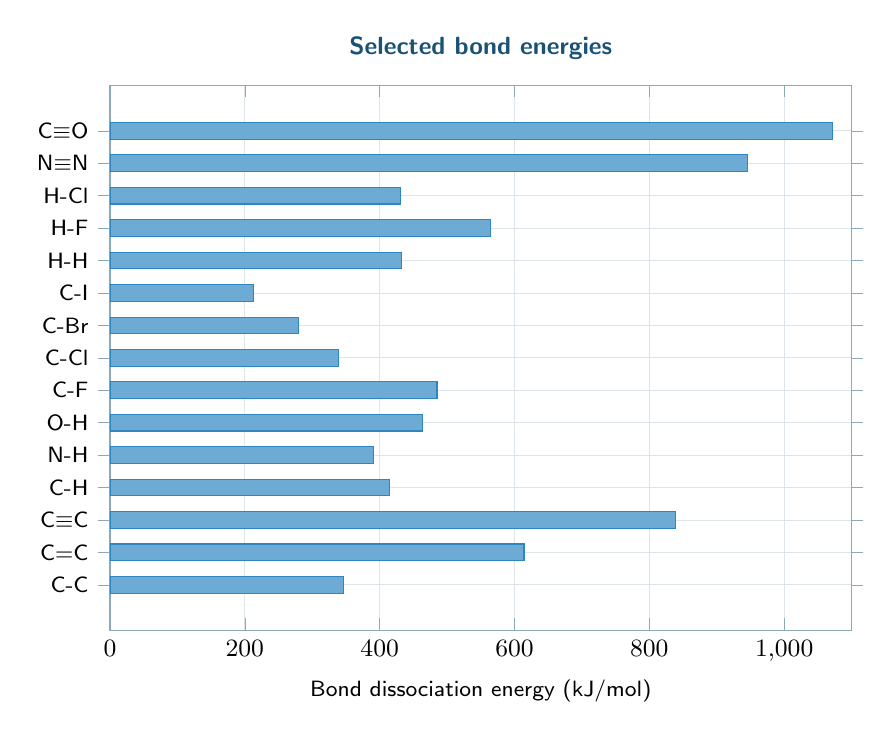
\begin{tikzpicture}[every node/.style={font=\sffamily\small}]
  \begin{axis}[
    xbar,
    width=11cm, height=8.5cm,
    xlabel={Bond dissociation energy (kJ/mol)},
    symbolic y coords={
      {C-C},{C=C},{C$\equiv$C},
      {C-H},{N-H},{O-H},
      {C-F},{C-Cl},{C-Br},{C-I},
      {H-H},{H-F},{H-Cl},
      {N$\equiv$N},{C$\equiv$O}
    },
    ytick=data,
    y tick label style={font=\sffamily\footnotesize},
    xmin=0, xmax=1100,
    xtick={0,200,400,600,800,1000},
    grid=major,
    grid style={line width=0.3pt, draw=JourneyColor!15},
    axis line style={color=JourneyColor!50},
    tick style={color=JourneyColor!50},
    title style={font=\sffamily\small\bfseries, color=JourneyColor},
    title={Selected bond energies},
    label style={font=\sffamily\footnotesize},
    bar width=6pt
  ]
    \addplot[fill=ModuleColor!70, draw=ModuleColor] coordinates {
      (346,{C-C})
      (614,{C=C})
      (839,{C$\equiv$C})
      (414,{C-H})
      (391,{N-H})
      (463,{O-H})
      (485,{C-F})
      (339,{C-Cl})
      (280,{C-Br})
      (213,{C-I})
      (432,{H-H})
      (565,{H-F})
      (431,{H-Cl})
      (945,{N$\equiv$N})
      (1072,{C$\equiv$O})
    };
  \end{axis}
\end{tikzpicture}
\end{center}

Key trends:
\begin{itemize}[nosep, leftmargin=2em]
  \item \textbf{Bond order matters}: single $<$ double $<$ triple
        (C--C: 346; C=C: 614; C$\equiv$C: 839 kJ/mol).
  \item \textbf{Bond polarity}: C--F (485 kJ/mol) is much
        stronger than C--I (213 kJ/mol) in the same column ---
        the more electronegative fluorine pulls harder.
  \item \textbf{N$\equiv$N (945 kJ/mol)} is among the strongest
        known bonds --- this is why atmospheric nitrogen is
        so inert, and why the Haber process requires such
        extreme conditions to break it.
  \item \textbf{C$\equiv$O (1072 kJ/mol)} is the strongest
        known bond --- stronger than N$\equiv$N.

\end{itemize}

\subsection{Bond Length and Bond Order}

Bond length and bond energy are inversely correlated:
stronger bonds are shorter.

\begin{center}
\small
\begin{tabular}{lcccc}
\toprule
Molecule & Bond & Order & Length (pm) & Energy (kJ/mol) \\
\midrule
\ce{C2H6} & C--C & 1 & 154 & 346 \\
\ce{C2H4} & C=C  & 2 & 134 & 614 \\
\ce{C2H2} & C$\equiv$C & 3 & 120 & 839 \\
\ce{N2H4} & N--N & 1 & 147 & 163 \\
\ce{N2H2} & N=N  & 2 & 123 & 418 \\
\ce{N2}   & N$\equiv$N & 3 & 110 & 945 \\
\bottomrule
\end{tabular}
\end{center}

\vspace{0.5em}

The pattern: adding a bond electron pair draws the nuclei
closer and increases the holding force.
This is the qualitative essence of molecular orbital theory ---
electrons in bonding orbitals lower the energy and
shorten the bond.

\subsection{The Bonding Puzzle and Its Quantum Resolution}

Why does electron \emph{sharing} stabilise a molecule?

The classical view says: two neutral atoms, no net force.
The quantum view reveals three stabilising effects
when atoms approach:

\begin{namedconcept}{The Three Quantum Sources of Bond Stability}
\begin{enumerate}[nosep, leftmargin=2em]
  \item \textbf{Kinetic energy lowering} (particle-in-a-box).
        An electron shared between two nuclei occupies a
        larger effective space than one confined to a
        single atom.
        By the uncertainty principle / particle-in-a-box:
        larger space $\Rightarrow$ lower kinetic energy.
        This is the dominant effect at long range.

  \item \textbf{Increased electron-nucleus attraction}.
        When an electron is in the bonding region between
        two nuclei, it is attracted to \emph{both} simultaneously.
        This lowers the potential energy more than either
        nucleus alone achieves.

  \item \textbf{Electron exchange} (quantum mechanical).
        For identical or similar atoms, the electron
        cannot be said to ``belong'' to one nucleus.
        It exists in a superposition --- a bonding orbital
        that spans both atoms.
        The exchange energy is a purely quantum effect with
        no classical analogue; it is the difference between
        the quantum and classical descriptions.
\end{enumerate}

These three effects together overcome the nuclear-nuclear
and electron-electron repulsions at the equilibrium geometry.
\end{namedconcept}

\begin{problembox}
\begin{enumerate}[label=\textbf{\arabic*.}]
  \item \textbf{Reading potential energy curves.}

        The potential energy curve for \ce{Cl2} has:
        $r_0 = 199$ pm, $D_e = 242$ kJ/mol.
        For HCl: $r_0 = 127$ pm, $D_e = 431$ kJ/mol.

        \begin{enumerate}[label=(\alph*)]
          \item Which bond is shorter? Suggest a reason
                from the electronegativity difference.
          \item Which bond is stronger?
                Explain using both bond order and polarity.
          \item Estimate the force constant $k$ for \ce{HCl}
                using the approximation that near the
                minimum, the potential is approximately
                harmonic: $V \approx \frac{1}{2}k(r-r_0)^2$.
                (For a Morse potential,
                $k = 2D_e a^2$ where $a \approx 0.016$ pm$^{-1}$
                for HCl.)
                What is the vibrational frequency
                $\nu = \frac{1}{2\pi}\sqrt{k/\mu}$
                where $\mu$ is the reduced mass?
        \end{enumerate}

  \item \textbf{Using bond energies to estimate reaction enthalpies.}

        The reaction enthalpy can be estimated from
        bond energies:
        $\Delta H \approx \sum D(\text{bonds broken}) -
                          \sum D(\text{bonds formed})$

        Calculate $\Delta H$ for:
        \begin{enumerate}[label=(\alph*)]
          \item \ce{H2(g) + Cl2(g) -> 2HCl(g)}
          \item \ce{CH4(g) + Cl2(g) -> CH3Cl(g) + HCl(g)}
          \item \ce{N2(g) + 3H2(g) -> 2NH3(g)}
                ($D_\text{N-H} = 391$ kJ/mol)
          \item For (c), compare to the experimental value
                $\Delta H = -92$ kJ/mol.
                Why does the bond energy method give
                approximate rather than exact values?
        \end{enumerate}

  \item \textbf{The particle-in-a-box analogy.}

        Model the \ce{H2+} ion (one electron, two protons)
        as a particle in a box.
        \begin{enumerate}[label=(\alph*)]
          \item When the protons are far apart (say $r \gg r_0$),
                the electron is essentially in a box of
                width $a_0$ (one hydrogen atom).
                Ground state energy: $E_1 \propto 1/a_0^2$.
          \item When the protons are at the bond length
                ($r_0 = 106$ pm for \ce{H2+}), the electron
                can delocalise over both atoms.
                Model this as a box of width $2a_0$.
                Ground state energy: $E_1 \propto 1/(2a_0)^2$.
          \item What is the ratio of kinetic energies?
                Does this rough model predict binding?
          \item The actual bond energy of \ce{H2+} is
                255 kJ/mol, versus 432 kJ/mol for \ce{H2}.
                What does the extra electron in \ce{H2}
                contribute?
        \end{enumerate}
\end{enumerate}
\end{problembox}

\subsection*{Deep Problems}

\begin{deepbox}
\begin{enumerate}[label=\textbf{D\arabic*.}]

  \item \textbf{The virial theorem and chemical bonding.}

        For any system in equilibrium, the virial theorem states:
        \[
          \langle E_k \rangle = -\tfrac{1}{2}\langle E_p \rangle
          \qquad \text{(Coulomb forces)}
        \]
        where $\langle E_k \rangle$ is the average kinetic energy
        and $\langle E_p \rangle$ is the average potential energy,
        and the total energy is $E = \langle E_k \rangle + \langle E_p \rangle$.

        \begin{enumerate}[label=(\alph*)]
          \item Show that the virial theorem implies
                $E = -\langle E_k \rangle = +\tfrac{1}{2}\langle E_p \rangle$.
          \item When \ce{H2} forms from two H atoms,
                the total energy decreases by 432 kJ/mol.
                What happens to the kinetic energy?
                Does it increase or decrease?
          \item This seems paradoxical: the molecule is
                more stable (lower total energy) but the
                electrons are \emph{moving faster}
                (higher kinetic energy).
                Reconcile this using the virial theorem.
          \item The kinetic energy increase comes from
                the electron being more tightly ``confined''
                in the molecule than in separate atoms ---
                yet we said larger space lowers kinetic energy.
                Resolve this apparent contradiction.
                (Hint: the equilibrium geometry is a
                compromise between two competing effects.)
        \end{enumerate}

  \item \textbf{Why \ce{He2} doesn't exist but \ce{He2+} does.}

        \ce{He2} would have the configuration
        $(\sigma_{1s})^2 (\sigma^*_{1s})^2$
        (two bonding, two antibonding electrons).
        \ce{He2+} has $(\sigma_{1s})^2 (\sigma^*_{1s})^1$.

        \begin{enumerate}[label=(\alph*)]
          \item The bond order is defined as
                $\frac{1}{2}(\text{bonding} - \text{antibonding})$.
                Calculate the bond orders of \ce{H2},
                \ce{H2+}, \ce{He2}, and \ce{He2+}.
          \item Predict which of these species exist as stable
                bound molecules in their ground states.
          \item The bond energy of \ce{He2+} is 251 kJ/mol
                and its bond length is 108 pm.
                Compare to \ce{H2+} (255 kJ/mol, 106 pm).
                Why are these values so similar despite
                He having twice the nuclear charge of H?
          \item \ce{He2} has been detected in liquid helium
                at very low temperatures as a van der Waals
                complex (bound by $\sim 0.009$ kJ/mol,
                bond length $\sim 520$ pm).
                What holds this complex together if
                there is no covalent bond?
        \end{enumerate}

\end{enumerate}
\end{deepbox}

\subsection*{Reflection}

\begin{reflectionbox}
\begin{enumerate}[label=\textbf{R\arabic*.}]
  \item We said bonds exist because electrons can
        ``be in two places at once'' (delocalization).
        \textbf{Is this a physical explanation or a
        mathematical description?}
        Does saying ``the wave function extends over both
        atoms'' tell you \emph{why} the energy is lower,
        or just \emph{that} it is lower?

  \item The bond dissociation energy of N$\equiv$N is
        945 kJ/mol.
        This makes nitrogen gas extremely inert,
        protecting the atmosphere, but also making
        biological nitrogen fixation the bottleneck
        for all protein synthesis on Earth.
        \textbf{In what sense is the strength of a chemical
        bond a ``fact about the universe'' that shapes
        the conditions for life?}

  \item The distinction between ``ionic'' and ``covalent''
        is a simplification --- all bonds are quantum
        mechanical, and the categories are points on
        a continuum.
        \textbf{Why do we use these categories at all?}
        When is a simplification scientifically useful
        even if it is technically wrong?
\end{enumerate}
\end{reflectionbox}

\vspace{1.5em}
\begin{center}
\begin{tcolorbox}[enhanced, colback=DiscoveryColor!8, colframe=DiscoveryColor,
  width=0.88\textwidth, arc=3pt]
\centering\sffamily\small
\textbf{What we invented in this module.}\\[4pt]
We posed the central question of Journey~4: why do
electrically neutral atoms attract each other?
The answer is quantum mechanical.
Electrons shared between two nuclei occupy a larger
effective space, lowering their kinetic energy.
They are simultaneously attracted to both nuclei,
lowering the potential energy.
At the equilibrium bond length, these gains balance
the nuclear-nuclear repulsion.
This mechanism operates differently for ionic, covalent,
metallic, and intermolecular bonds ---
but all bonding ultimately traces to the same source:
the quantum mechanical behaviour of electrons in the
field of positive nuclei.
\end{tcolorbox}
\end{center}

\vspace{2em}
\noindent\textcolor{JourneyColor!40}{\rule{\textwidth}{0.6pt}}
\begin{center}
\textit{\sffamily\small
Module 4.1 complete. Continue to Module 4.2:\\
\textbf{Ionic Bonding: Electrostatics and the Born-Haber Cycle}.}
\end{center}

\end{document}